\documentclass[letterpaper, 12pt]{article}
\usepackage[letterpaper,margin=1in]{geometry}
\usepackage[english]{babel}
\usepackage{graphicx}
\usepackage{hyperref}
\usepackage{booktabs}
\usepackage[explicit]{titlesec}
\usepackage{fancyhdr}
\usepackage{inputenc}
\usepackage{enumitem,amssymb}
\usepackage{tikz}
\usetikzlibrary{arrows.meta}
\usetikzlibrary{calc}
\pagestyle{fancy}

\titleformat{\section}
  {\normalfont\Large\bfseries}{\thesection}{1em}{\hyperlink{sec-\thesection}{#1}
\addtocontents{toc}{\protect\hypertarget{sec-\thesection}{}}}
\titleformat{name=\section,numberless}
  {\normalfont\Large\bfseries}{}{0pt}{#1}
  
\titleformat{\subsection}
  {\normalfont\large\bfseries}{\thesubsection}{1em}{\hyperlink{subsec-\thesubsection}{#1}
\addtocontents{toc}{\protect\hypertarget{subsec-\thesubsection}{}}}
\titleformat{name=\subsection,numberless}
  {\normalfont\large\bfseries}{\thesubsection}{0pt}{#1}

\titleformat{\subsubsection}
  {\normalfont\large\bfseries}{\thesubsubsection}{1em}{\hyperlink{subsec-\thesubsubsection}{#1}
\addtocontents{toc}{\protect\hypertarget{subsec-\thesubsubsection}{}}}
\titleformat{name=\subsubsection,numberless}
  {\normalfont\large\bfseries}{\thesubsubsection}{0pt}{#1}


\newlist{todolist}{itemize}{2}
\setlist[todolist]{label=$\square$}
\usepackage{pifont}
\newcommand{\cmark}{\ding{51}}%
\newcommand{\xmark}{\ding{55}}%
\newcommand{\done}{\rlap{$\square$}{\raisebox{2pt}{\large\hspace{1pt}\cmark}}%
\hspace{-2.5pt}}
\newcommand{\wontfix}{\rlap{$\square$}{\large\hspace{1pt}\xmark}}



\begin{document}


\begin{titlepage}
\centering
	{\LARGE RoboJackets IGVC}\\
	\vspace{1cm}
	{\Large IGVC Logic Board 2019}\\
	\vfill
	{\large Created at November 18, 2017}\\
	\vspace{1cm}
	{\large Last Edited at \today\par}
\end{titlepage}

\tableofcontents

\pagebreak
% \section*{Todo Lists}
% \begin{todolist}
%   \item[\done] Update system diagram
%   \item[\done] Update relevant info
%   \item Schematics?
%   \item[\done] Sabertooth pinout
%   \item[\done] Indicator meaning
%   \item Lidar lites
%   \item Firmware
%   \item[\done] Estop system
% \end{todolist}

% \pagebreak

\section{Overview}
This document documents the functionality of the Logic Board (previously referred as \emph{motor board},
or Motor and Light Control Board in the year 2017 - 2018) in the IGVC subteam in \emph{RoboJackets}.
This document aims at providing the reader with the board's capability and limitation. \vspace{6pt}\\
The logic board is the interface between IGVC's software team and her actuators. Software team completes
path and motion planning in the onboard computer and sends driving commands via Ethernet to mbed on the Logic
Board, which then converts to Serial message to the Sabetooth motor controller.\\
% \begin{figure}[h]
%     \centering
%     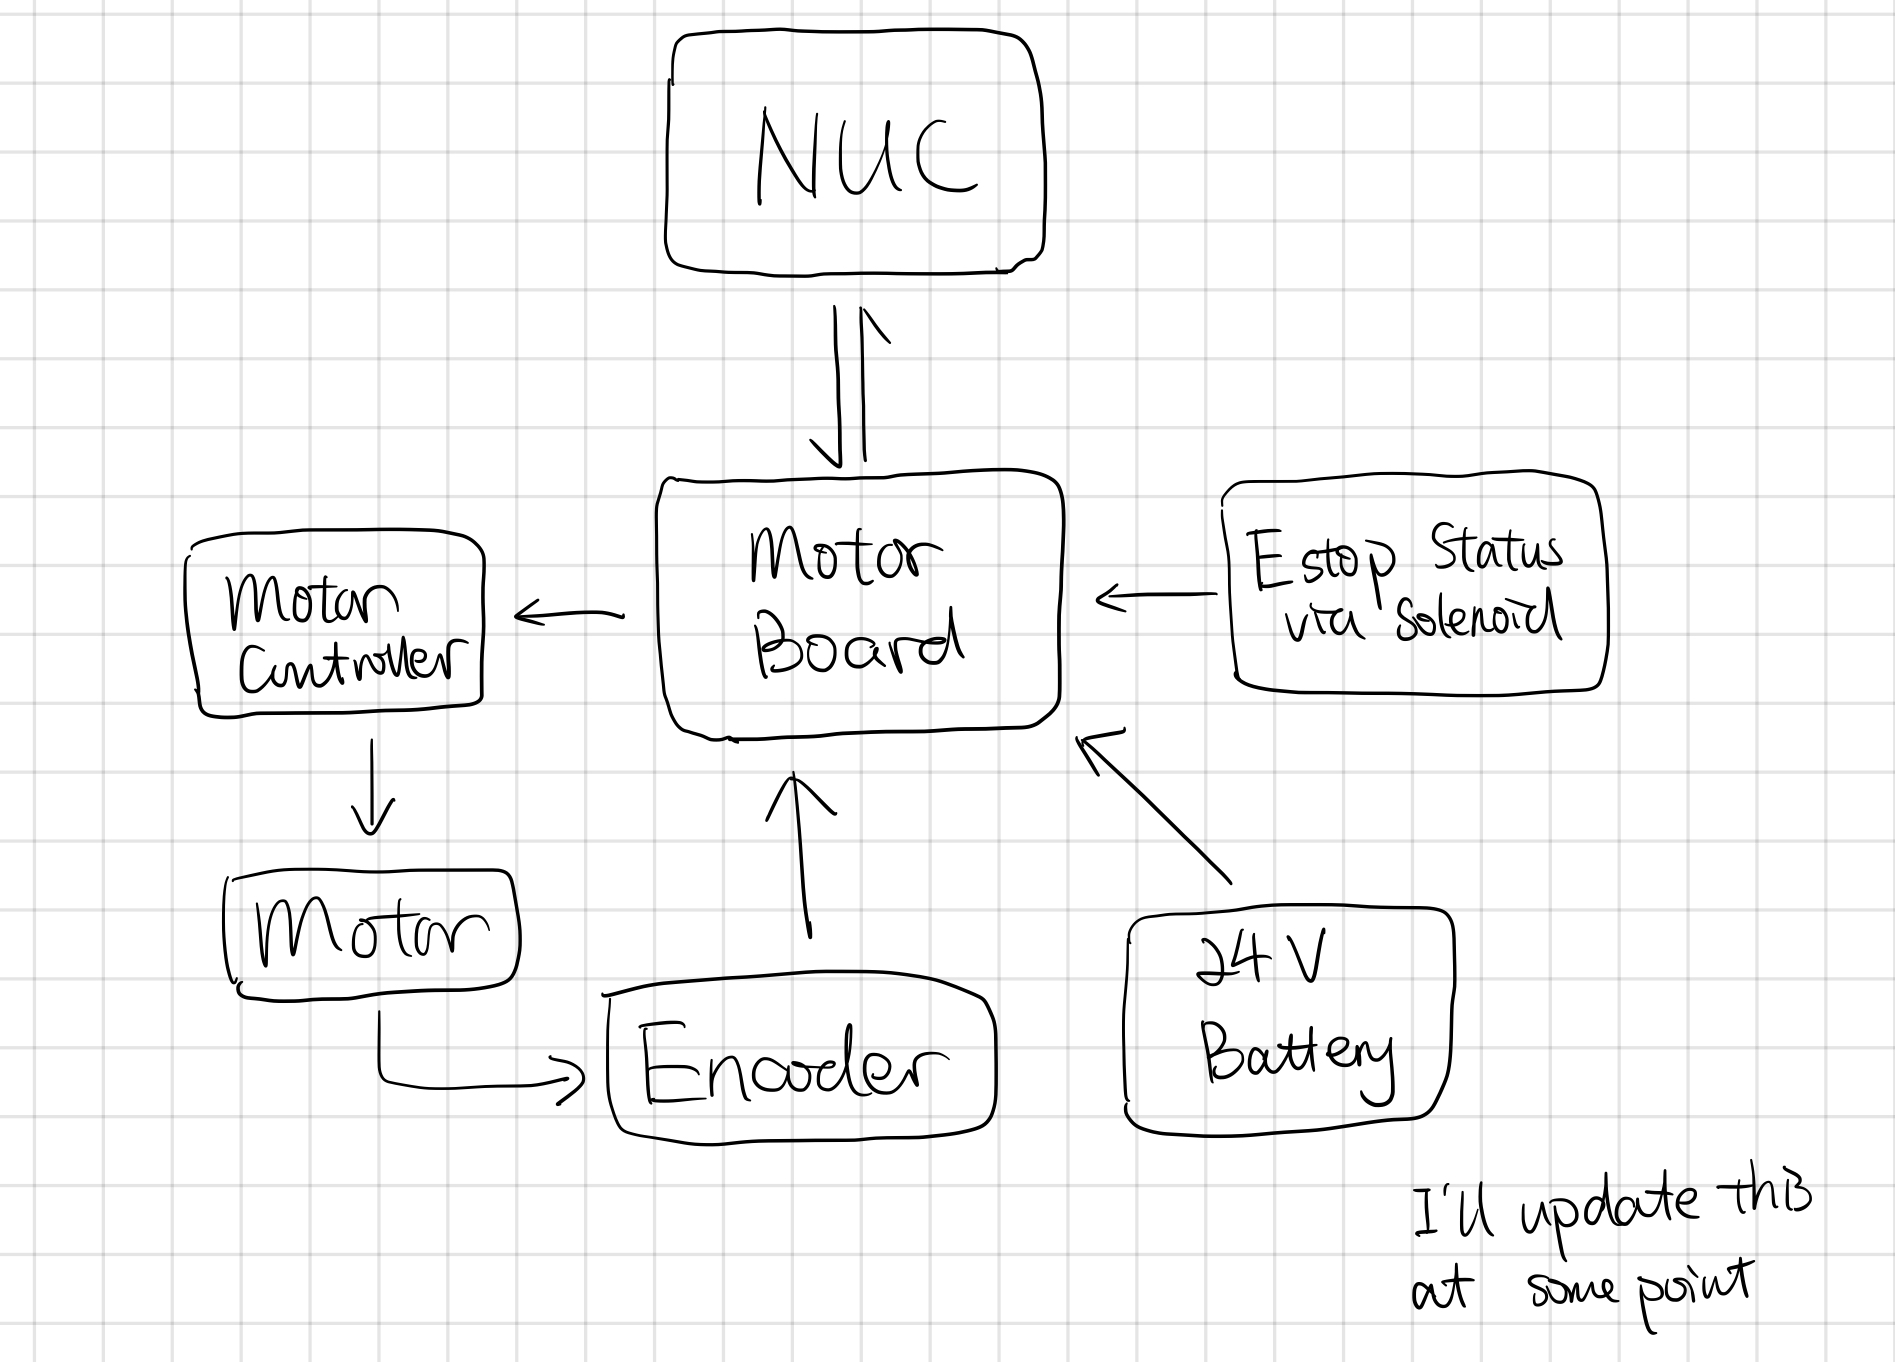
\includegraphics[width=0.7\textwidth]{UpandLow.png}
%     \caption{motor board's Data Input and Output}
%     \end{figure}

\begin{figure*}[th]
    \centering
    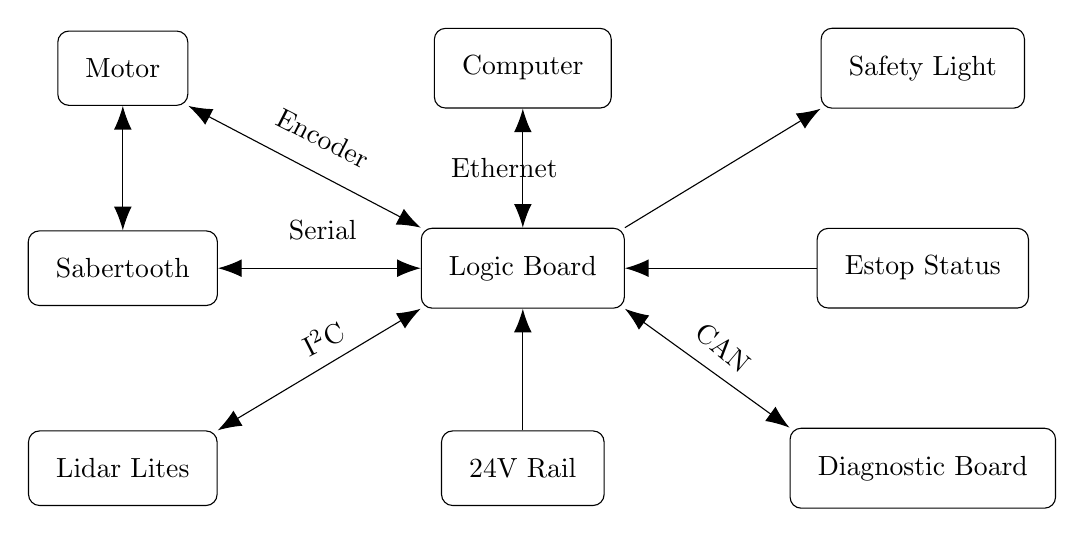
\begin{tikzpicture}[inner sep=1em]
        \node[anchor=center, draw=black, rounded corners,] (pc) at (0in, 0in) {Computer};
        \node[anchor=center, draw=black, rounded corners,] (logic) at (0in, -1in) {Logic Board};
        \draw[{Latex[length=3mm]}-{Latex[length=3mm]}](pc.south)--(logic.north);
        \node[anchor=west] (ethernet) at (-0.5in, -0.5in) {Ethernet};

        \node[anchor=center, draw=black, rounded corners,] (sabertooth) at (-2in, -1in) {Sabertooth};
        \draw[{Latex[length=3mm]}-{Latex[length=3mm]}] (sabertooth.east)--(logic.west);
        \node[anchor=south] (serial) at (-1in, -1in) {Serial};
        \node[anchor=center, draw=black, rounded corners,] (motor) at (-2in, 0in) {Motor};
        \draw[{Latex[length=3mm]}-{Latex[length=3mm]}] (sabertooth.north)--(motor.south);
        \draw[{Latex[length=3mm]}-{Latex[length=3mm]}] (motor.south east) -- (logic.north west);
        \node[anchor=center, rotate=-27] at (-1in, -0.35in) {Encoder};
 
        \node[anchor=center, draw=black, rounded corners,] (safety) at (2in, 0in) {Safety Light};
        \draw[{Latex[length=3mm]}-] (safety.south west)--(logic.north east);

        \node[anchor=center, draw=black, rounded corners,] (estop) at (2in, -1in) {Estop Status};
        \draw[-{Latex[length=3mm]}] (estop.west)--(logic.east);

        \node[anchor=center, draw=black, rounded corners,] (diag) at (2in, -2in) {Diagnostic Board};
        \draw[{Latex[length=3mm]}-{Latex[length=3mm]}] (logic.south east)--(diag.north west);
        \node[anchor=center, rotate=-40] at (1in, -1.4in) {CAN};

        \node[anchor=center, draw=black, rounded corners,] (vrail) at (0in, -2in) {24V Rail};
        \draw[-{Latex[length=3mm]}] (vrail.north)--(logic.south);

        \node[anchor=center, draw=black, rounded corners,] (lidar) at (-2in, -2in) {Lidar Lites};
        \draw[{Latex[length=3mm]}-{Latex[length=3mm]}] (lidar.north east)--(logic.south west);
        \node[anchor=center, rotate=27] at (-1in, -1.35in) {I$^2$C};

    \end{tikzpicture}
    \caption{Logic board's Data Input and Output}
\end{figure*}
    


The primary function of the logic board contains the following:
\begin{itemize}
    \item Relay motor commands from software stack to motor controller and perform control algorithm in the process.
    \item Monitoring battery voltage and estop status, relay both to software stack.
    \item Communicate with the rest of electrical system and relay necessary information to the software stack.
\end{itemize}
Previous version of Logic board (motor and light) contains legacy interface for Open Source Motor Controller (OSMC)
which has been removed from the current version.

The motor board is controlled by an mbed NXP LPC1768 microcontroller development board (referred as mbed in the following). More details here: \url{https://os.mbed.com/platforms/mbed-LPC1768/} \vspace{6pt}\\
\pagebreak

\section{Hardware}
The motor board is designed using AutoDesk EagleCAD. Currently the PCB design files can be find under branch \texttt{rev/logic}
of \texttt{igvc-electrical} repository. Here's a link to master branch: \url{https://github.com/RoboJackets/igvc-electrical/}.

\subsection{Power System}
Four voltage level runs through this board. 
\begin{table}[h]
  % \boxed{
    \caption{Summary of functions of Voltage Levels}
    \centering
    \begin{tabular}{p{3cm}p{4cm}p{4cm}}
    \toprule
    Level ($V$)  & Direct Input Source & Maximum Ampere \\
    \midrule
    24V  & Robot Battery & ? \\
    12V  & 12V Rail & 3A  \\
    5V  & 12-5 Regulator & 1A \\
    3V3 & 5-3.3 Regulator & 300mA \\
    \bottomrule
    \end{tabular}
  % }
\end{table}

24V does not have a power plane on the motor board. The sole purpose of having 24V running
through this board is for battery voltage monitor. 24V will be divided between a 4.7k and
a 510 $\Omega$ resistor to achieve a voltage level of maximum 2.34V. The mbed reads in this value
from Analog pin \texttt{p19} to monitor the battery voltage. 

\begin{equation}
    V_{batt} = V_{in} \times 3.3 \times (4700 + 510) / 510 
\end{equation}

\vspace{1em}The rest of the power planes are shown on Figure \ref{fig:pwr_plane}.\\

12V plane is the main power source for the motor board. 12V plane powers the 5V plane via
12V-5V regulator (T1). LED under-glow, flood light and safety light resides on this power
plane. Each with components of sufficient ampere rating. \\

5V plane powers the mbed, encoder and the USB port to the PC. 5V plane powers the 3V3 plane
via the 5V-3V3 regulator, while the 3V3 plane only powers the imu and the ethernet port. \\

\begin{figure}[h]
\centering
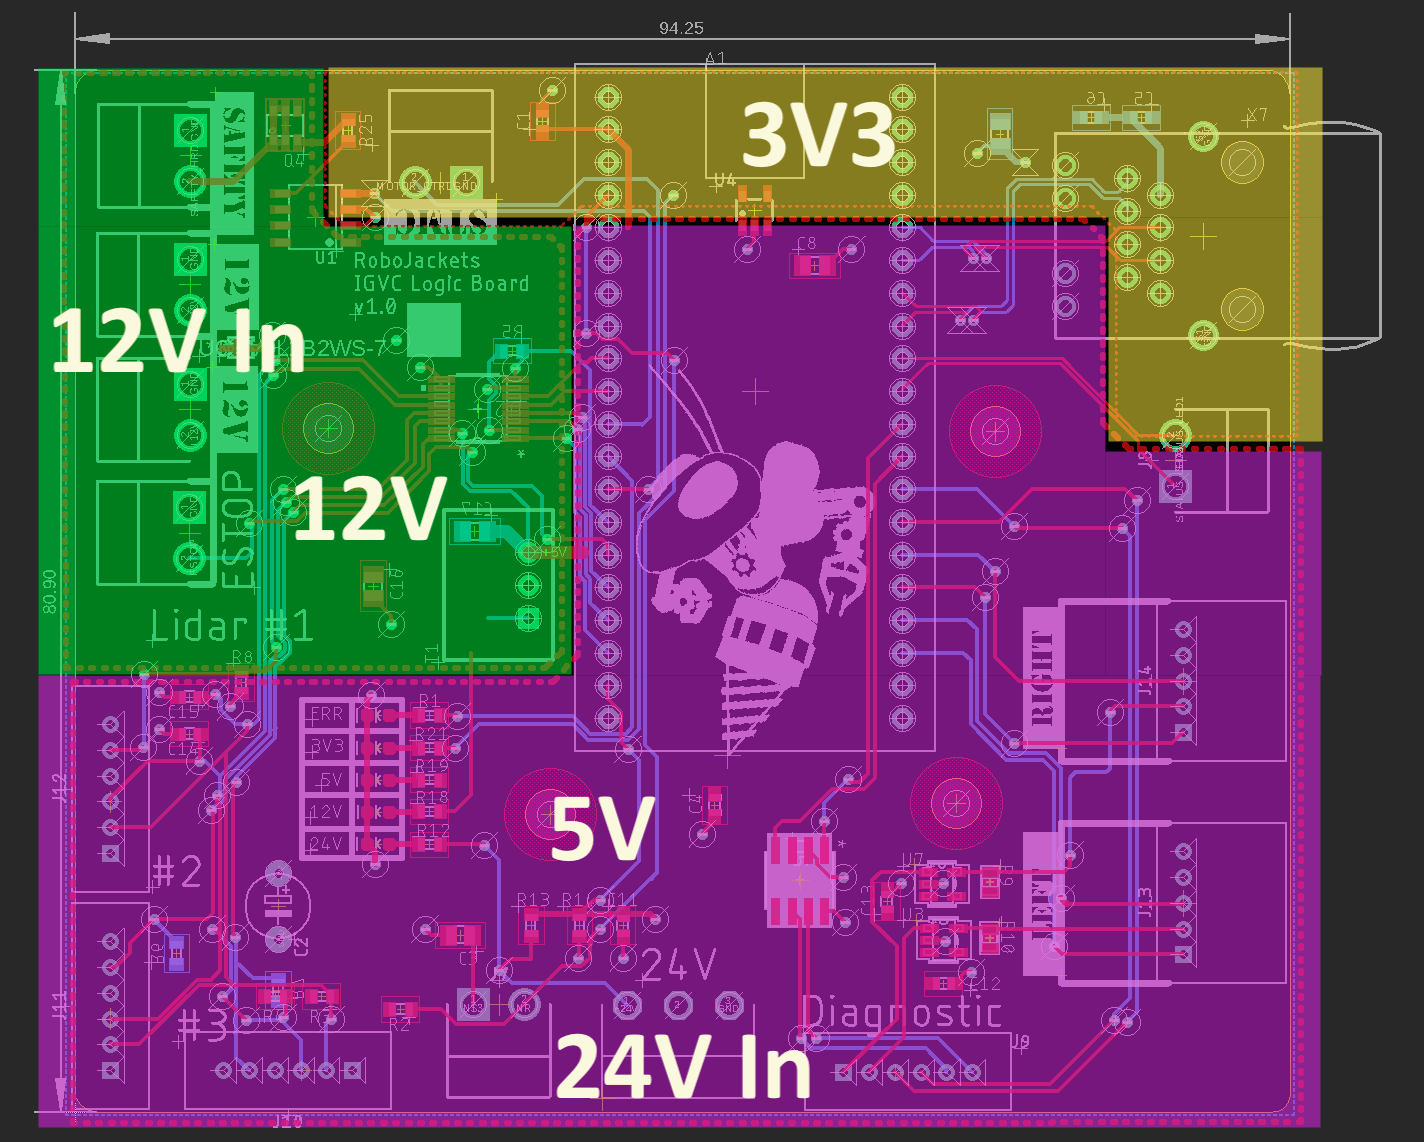
\includegraphics[width=0.6\textwidth]{img/pwr_plane.png}
\caption{Power Plane Indication} \label{fig:pwr_plane}
\end{figure}

Each power plane has a dedicated LED indicator, indicating that this specific power plane
has been powered up. Notice that when \textbf{only} USB(either to mbed or X1 port) is connected,
without 12V power, 12V LED may still light up. This is caused by the internal design of 12-5 regulator.
The fact that 12V LED will light up only dimly suggest that 12V plane does not run 12V at this point.
It is \textbf{STRONGLY DISCOURAGED} to power the logic board solely by the mbed or USB port.


\begin{figure}[h]
  \centering
  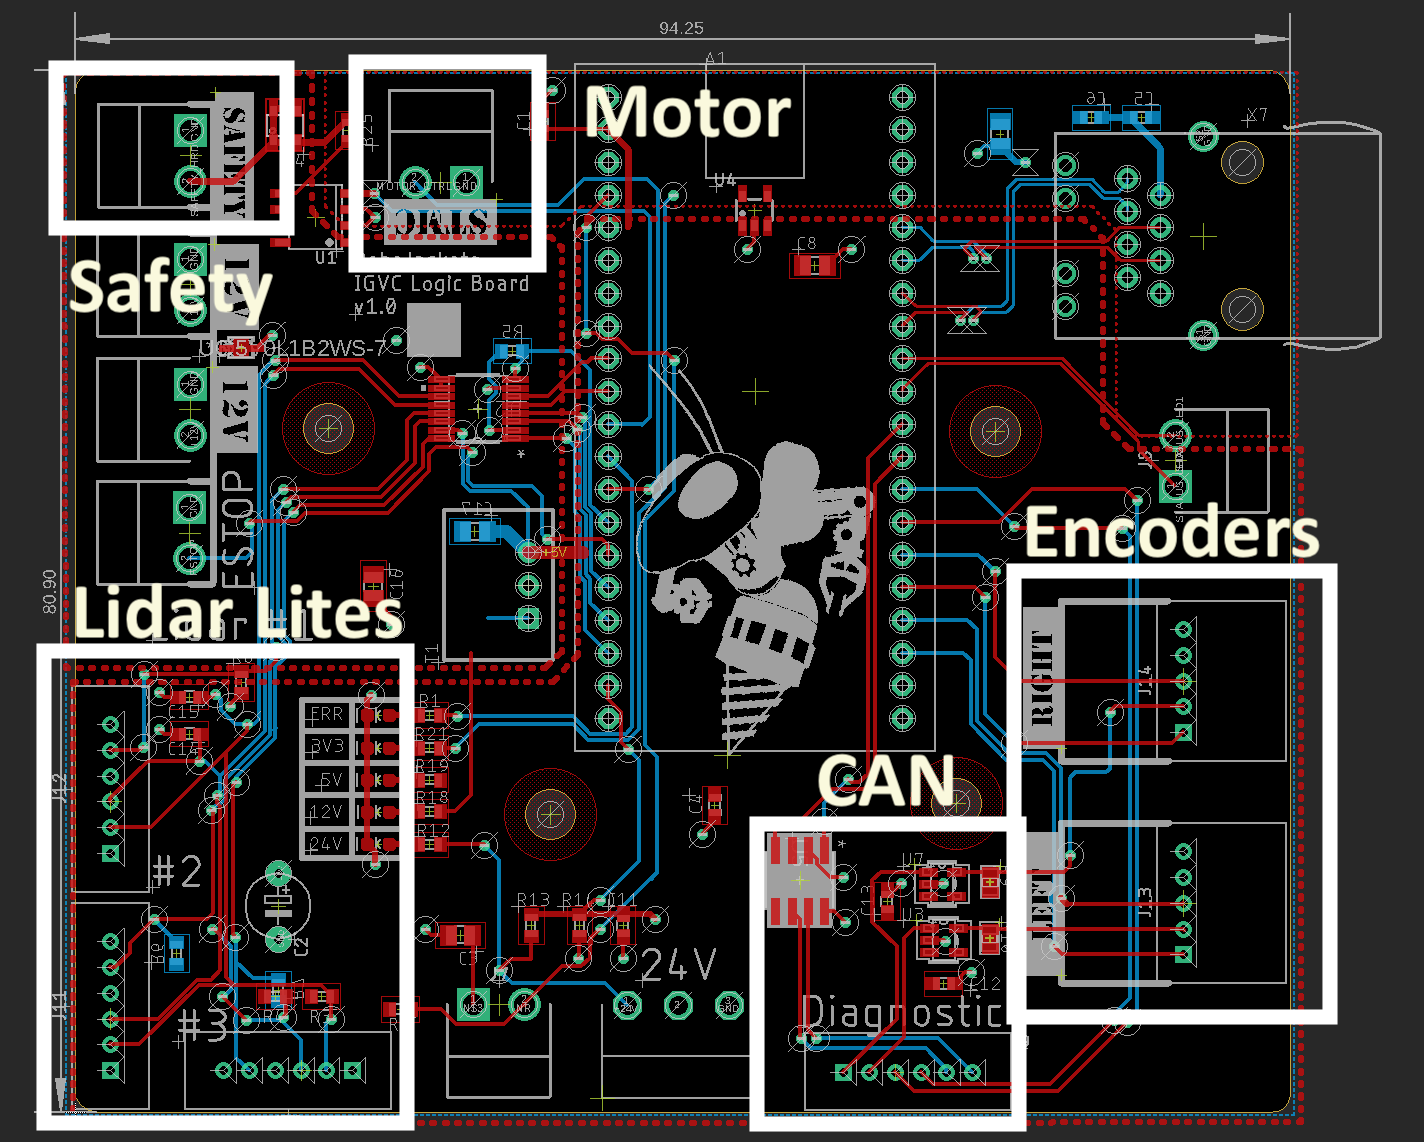
\includegraphics[width=0.6\textwidth]{img/conns.png}
  \caption{Power Plane Indication} \label{fig:conns}
  \end{figure}

\subsection{Motor Control}

The connection port on the board can be found labeled in Figure \ref{fig:conns}.

Logic board interface with an off-the-shelf motor controller to control the IGVC motors. Logic board itself
does not run any high power current through the board. Motors on the IGVC robot is controlled by the
Sabertooth 2x60 A motor controller. Data sheets can be found here:
\url{https://www.dimensionengineering.com/products/sabertooth2x60}.\\

Motor board communicate with Sabertooth motor controller via a one-line serial communication
(the "Simplified Serial Communication" Mode). Only \textbf{tx} line on mbed is used, Sabertooth
does not send back any data and \textbf{rx} line on mbed may leave as not connected and used
for other purposes.\\

Port S1 is used for connection to sabertooth motor controller. The serial line connects to port
S1 on the sabertooth motor controller. For switch and other specific configurations, please refer
to the Sabertooth data sheet listed earlier. \\

The Logic board receives motor measurements through optical rotary encoders each with channel A and B.
Every change\footnote{or rise or fall, depending in firmware implementation} in tick would trigger an interrupt
function in the mbed code that increments the counter for angular displacement calculation. 

\subsection{Light Control}
Logic board controls the indicator light.\\

The indicator light is required by the competition rule that it should display different pattern
with regards to whether the robot is powered on or not and in autonomous mode or not. 
Logic board controls whether the light safety light is in flashy mode. The control signal comes from
the software stack.

Previously the motor and light Board contains a functionality for controlling underglows. This has been
moved offboard to a standalone board.

\subsection{Lidar Lites}

The lidar lites are for the concept of virtual bumper. Virtual bumper serves as an extra layer of sanity check to inform
the software stack that the robot is getting dangerously close to an obstacle. \\

The virtual bumper are formed via three Lidar Lites v3 water proof version that points outwards in forward, left and right 45 degrees fashion.
The are linked to the logic board via three six pin connectors and via I$^2$C protocol. Note that three lidar lites shares the same initial 
device address for I$^2$C therefore the design is to sequentially power them up and change the device address so that informations to every device
maybe retrieved. \\

Note that the overwritten device address would be \textbf{reset} after every power cycle. It is necessary to make the sequential power up part of the
regular routine of mbed code startup cycle. 

\subsection{Controller Area Network}

Controller Area Network, or CAN, are adapted on the board so that multiple boards may share the same message bus without the fear that the failure
of any board would bring down the entire network. 

Conventionally, for any micro-controller to join up in a CAN network, it would require that board to talk with a CAN controller, which then in turn
talk to the CAN transceiver that communicate on the CAN bus. The mbed has a built-in CAN controller and only a transceiver is present on the board. 
Be advised that the design of other board would require both a CAN controller and a CAN transceiver. 

\pagebreak

\section{Firmware}
Logic board firmware is currently undergoing an overhaul lead by Dallas Downing. You can find the code in 
\url{https://github.com/RoboJackets/igvc-firmware/tree/master/src/mbed}. mbed communicates with the computer via Ethernet
and Google's Protobuf library. 

\section{Control}
\subsection{PID Algorithm}
For software team to have a reliable localization, control over exact speed of motors are required.\\

Such control is done through PID algorithm in the motor board. PID stands for Proportional-Integral-Derivative controller. It operates on the idea that the output is changed based on the proportional, derivative and integral of difference between desired speed and actual speed over a certain $dT$. Details see \url{https://en.wikipedia.org/wiki/PID_controller}\\

Parameter values P, I and D need to be tuned for every different system. Increase proportional term value will increase the speed of the control system response, but will enlarge the overshoot and cause oscillation. Increase derivative term will cause the control system to react more strongly to changes in the error term, but will make the system unstable if the feedback signal is noisy. Increase integral term will sum overtime and drive the Steady-state error to zero, but will also increase the risk of a phenomenon called integral windup. \\

In short, PID need to be tuned, manually, especially if you're reading this document, since the robot probably has gone through a major remake and the system transfer function for the gear box + robot has changed.

\subsection{Emergency Stop}
In the event of IGVC robot goes terminator, absolute control over motor is required.\\

Emergency stop is the hardware stop for our robot that will physically cut power to motors,
done via a solenoid with diode magic circuits. The significance of Estop to the logic board
is that if the motors are cut power and motor board is still running PID algorithm, PID will
think power increase is not resulting in reduction of error, thus increase power output and
eventually reach maximum. When the robot is re-enabled, such error may cause robot to tip over. \\

A port is added to the motor board to accommodate this issue. Port marked "Estop" is for monitoring
estop status. In current electrical system design, when robot is stoped, this port will receive a +5V
signal and will be left floating when robot is enabled. This floating signal is complemented by mbed
pin's internal pull down configuration. 

This signal is further relayed to software stack in \texttt{robot enabled}. The logic board itself
does not perform any functionality in the estop system and does not need to be onboard the robot to test
the estop system.

\section{Miscellaneous}
\subsection{Expected Future Usage}
When the motor board was first designed, we left a ethernet port that was eventually utilized by IGVC for their
stability over simulated Serial port. So much that we have retired the USB port on the logic board. It is hard to
imagine what can be used for the future version of the logic board, since the control board now requires a major
revision as IGVC move towards swerve drive. There are always things to be done on the software level. It is not
hard to implement sensor fusion on the mbed and people should consider that possibility. After all, it is only
a small  embedded platform, robustness is of the most importance.

\subsection{Special Regards}
The author would like to thank Evan Peterson and Ryo Osawa from RoboJackets RoboCup team for their
awesome help in reviewing the design of board and much helpful advice. He would also like to thank
Jason Gibson from RoboJackets IGVC software team for his time in debugging Serial communication
problems with NUC.  

\subsection{Legacy Interfaces}
\textbf{NOT PRESENT IN LOGIC BOARD!}\\
IGVC robot Woodi (Year 2016 - 2017) and her predecessors used 4 Open Source Motor Controller (Referred as OSMC in the following) to control its motors. Current IGVC robot Jessi no longer uses OSMCs, yet a legacy port is reserved on the motor board in case for any unexpected incident. \vspace{6pt}\\
OSMCs are essentially H-bridge DC motor control circuits. Due to the specific design of OSMC, both switches on the high side of H-bridge are hard-wired to \textbf{CLOSED}. Therefore speed and direction control solely depends on the value of low side switches (see OSMC datasheet for specific control logic). The mbed has direct control over the low-side switches via PWMOut pins from p21 to p24. Be advised that one should \textbf{NEVER} set two low switches on the same H bridge to \textbf{CLOSED} at \textbf{ANY TIME}. \vspace{6pt}\\
The motor board used 2 Optoisolators chips to help control the low-side switches. Optoisolators keeps the motor board circuits electrically separated from the motor power circuits. Such design helps to protect the mbed from the fluctuation caused by motors. Although \emph{technically}, the mbed and the motor will still share the same ground level, having them not directly electrically connected through the motor board gives more time for the rest of the system to damp the fluctuation and protect the mbed. \vspace{6pt}\\
OSMC datasheets can be found here:\\
\url{http://www.robotpower.com/downloads/osmc3-22sch-clean.pdf}\\

\end{document}